\documentclass{beamer}

\beamertemplatenavigationsymbolsempty

\usepackage[utf8]{inputenc}
\usepackage{bm}
\graphicspath{ {./graphics/} }
\usepackage{amssymb}
\usepackage{amsmath}
\usepackage{amsfonts}
\usepackage{color}
\usepackage{isotope}

\newcommand{\be}{$\beta$}
\newcommand{\al}{$\alpha$}
\newcommand{\li}{\isotope[8]{Li}\xspace}
\newcommand{\ber}{\isotope[8]{Be}\xspace}


%Information to be included in the title page:
\title{TITEL}
\subtitle{En anden fin titel}
\author{Anders Holst Rasmussen}
\date{28. Juni, 2021}

\mode<presentation> {
	\usetheme{CambridgeUS}
	\usecolortheme{seahorse}
	%\setbeamercovered{transparent}
}

\AtBeginSection[]
{
	\begin{frame}
		\frametitle{Oversigt}
		\tableofcontents[currentsection]
	\end{frame}
}

\begin{document}
\frame\titlepage
\section{Introduktion}

\begin{frame}{\be-henfald}
	To typer:
	\begin{align*}
	\onslide<2->{&\beta^+:\quad p\rightarrow n + e^+ + \nu_e\\}
	\onslide<2->{&\beta^-:\quad n\rightarrow p + e^- + \bar{\nu_e}}
	\end{align*}
	\onslide<3->{Forskellige Q-værdier:}
	\begin{align*}
	\onslide<4->{&Q_{\beta^+} = \left[ m (\isotope[A][Z]{X}) - m(\isotope[A][Z-1]{X'})  		 \right] c^2\\
	&Q_{\beta^-} = \left[ m (\isotope[A][Z]{X}) - m(\isotope[A][Z+1]{X'}) -2m_e  \right] c^2}
	\end{align*}
\end{frame}

\begin{frame}{\be-henfald}
	Tilladte overgange:
	\begin{equation*}
	\onslide<2->{\Delta J = 0, \pm1,\ \Delta T = 0, \pm 1,\ \text{og}\ \Delta \pi = 0}
	\end{equation*}
	\onslide<3->{Spin, paritiet og isospin: $J^\pi ; T$}
	\onslide<4->{
		\begin{figure}
			\centering
			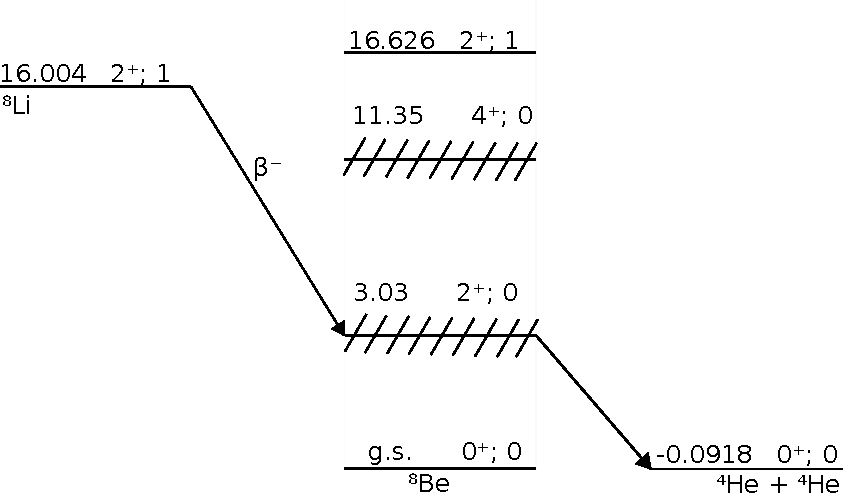
\includegraphics[width=.6\columnwidth]{../figures/DecayScheme.pdf}
		\end{figure}
	}
\end{frame}

\begin{frame}{\al-henfald}
	Udsendelsen af \al-partikel\\
	\onslide<2->{Q-værdi:
		\begin{equation*}
			Q_\alpha = \left[ m\left(^A_Z X\right) - m\left( ^{A-4}_{Z-2} X' \right) -m_\alpha \right]c^2
		\end{equation*}
	}
\end{frame}
\section{Eksperimentel opsætning}

\begin{frame}{Eksperimentel opsætning}
	\begin{columns}
		\column{0.4\textwidth}
		\begin{figure}
			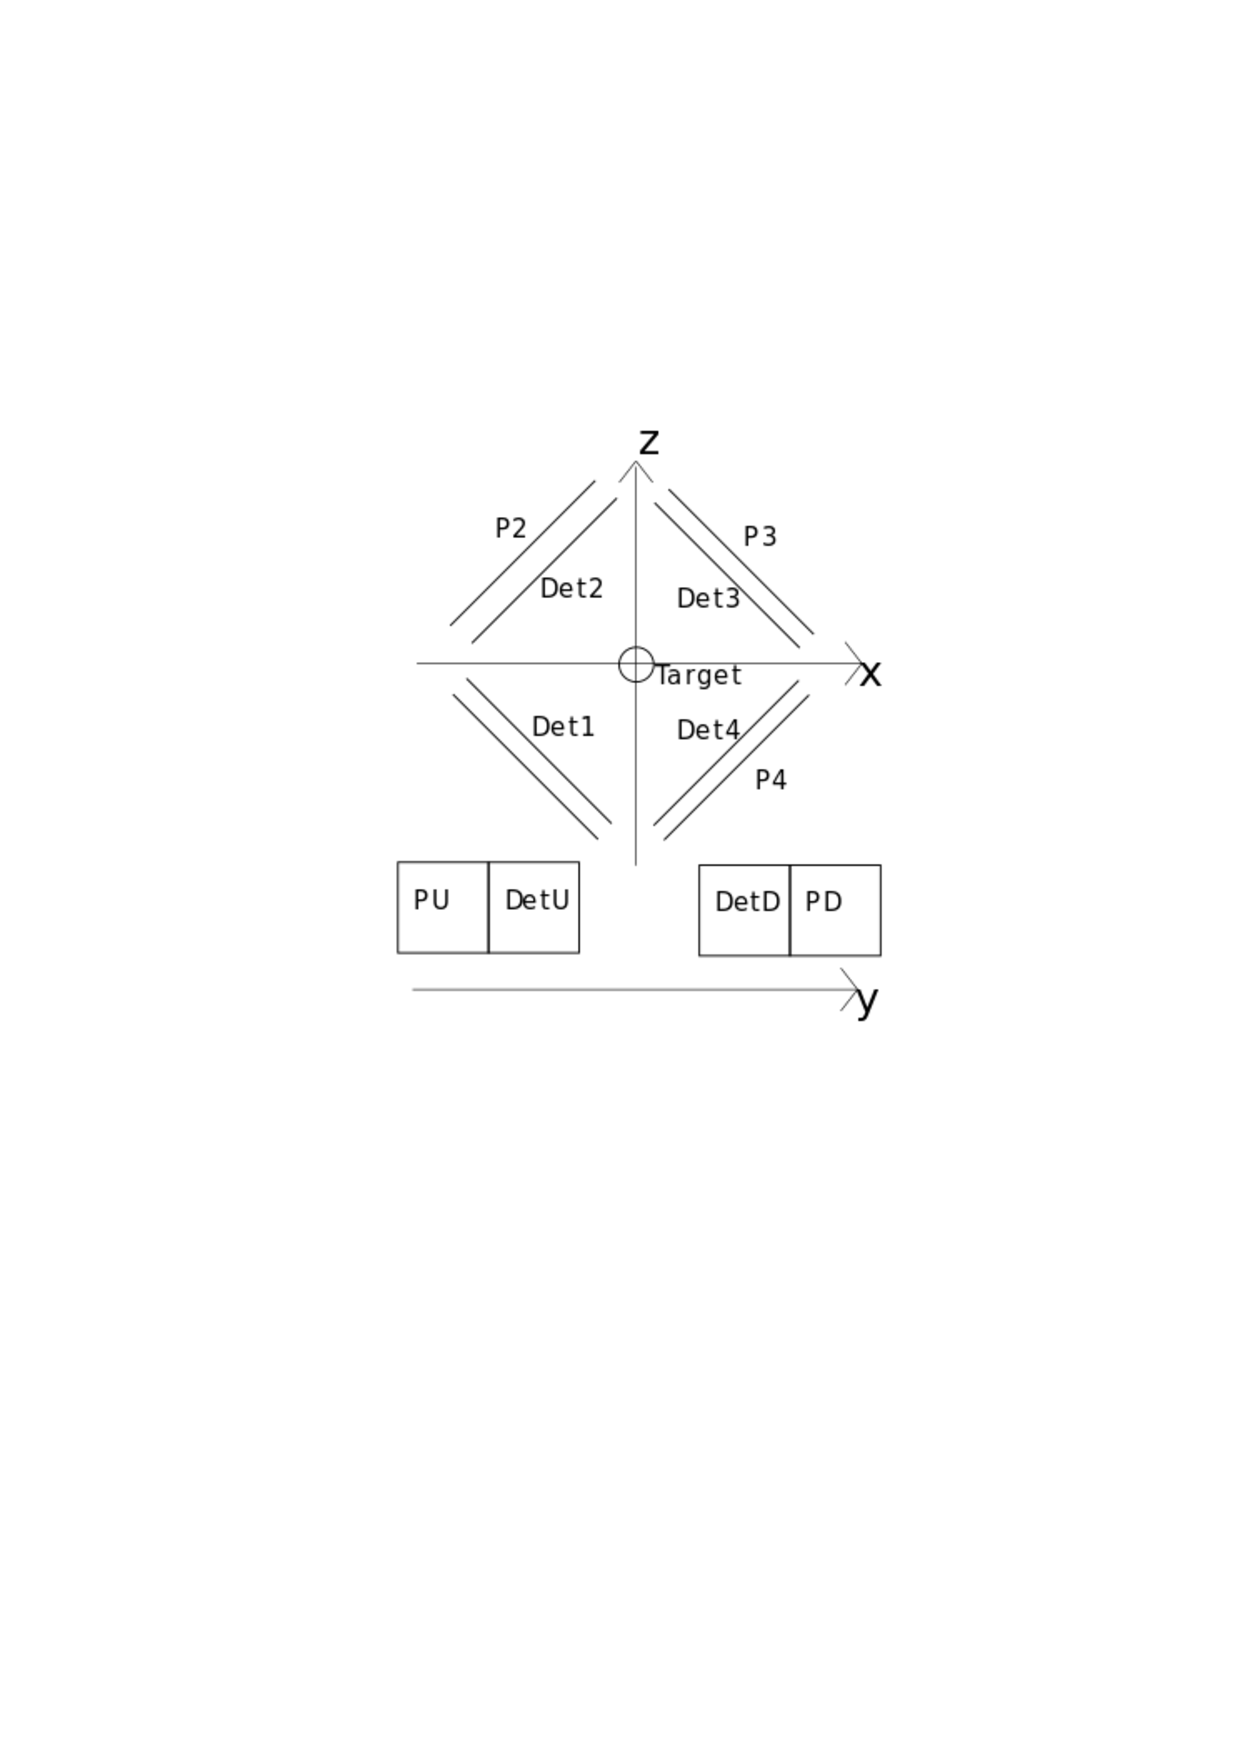
\includegraphics[width=\columnwidth]{../figures/opstilling_better.pdf}
		\end{figure}
		
		\column{0.6\textwidth}
		\small
		\begin{table}
			\begin{tabular}{ll|ll}
				Detektor & Tykkelse {[}$\mu$m{]}  & PAD & Tykkelse{[}$\mu$m{]} 	\\ \hline
				Det1     & 67                     & n/a & n/a                   \\
				Det2     & 1002                   & P2  & 1036                  \\
				Det3     & 65                     & P3  & 1497                  \\
				Det4     & 60                     & P4  & 1490                  \\
				DetU     & 60                     & PU  & 1498                  \\
				DetD     & 1043                   & PD  & 1038                 
			\end{tabular}
		\end{table}		
	\end{columns}


\end{frame}

\begin{frame}{Eksperimentel opsætning}
	\begin{columns}
		\column{0.49\textwidth}
		\begin{figure}
			\centering
			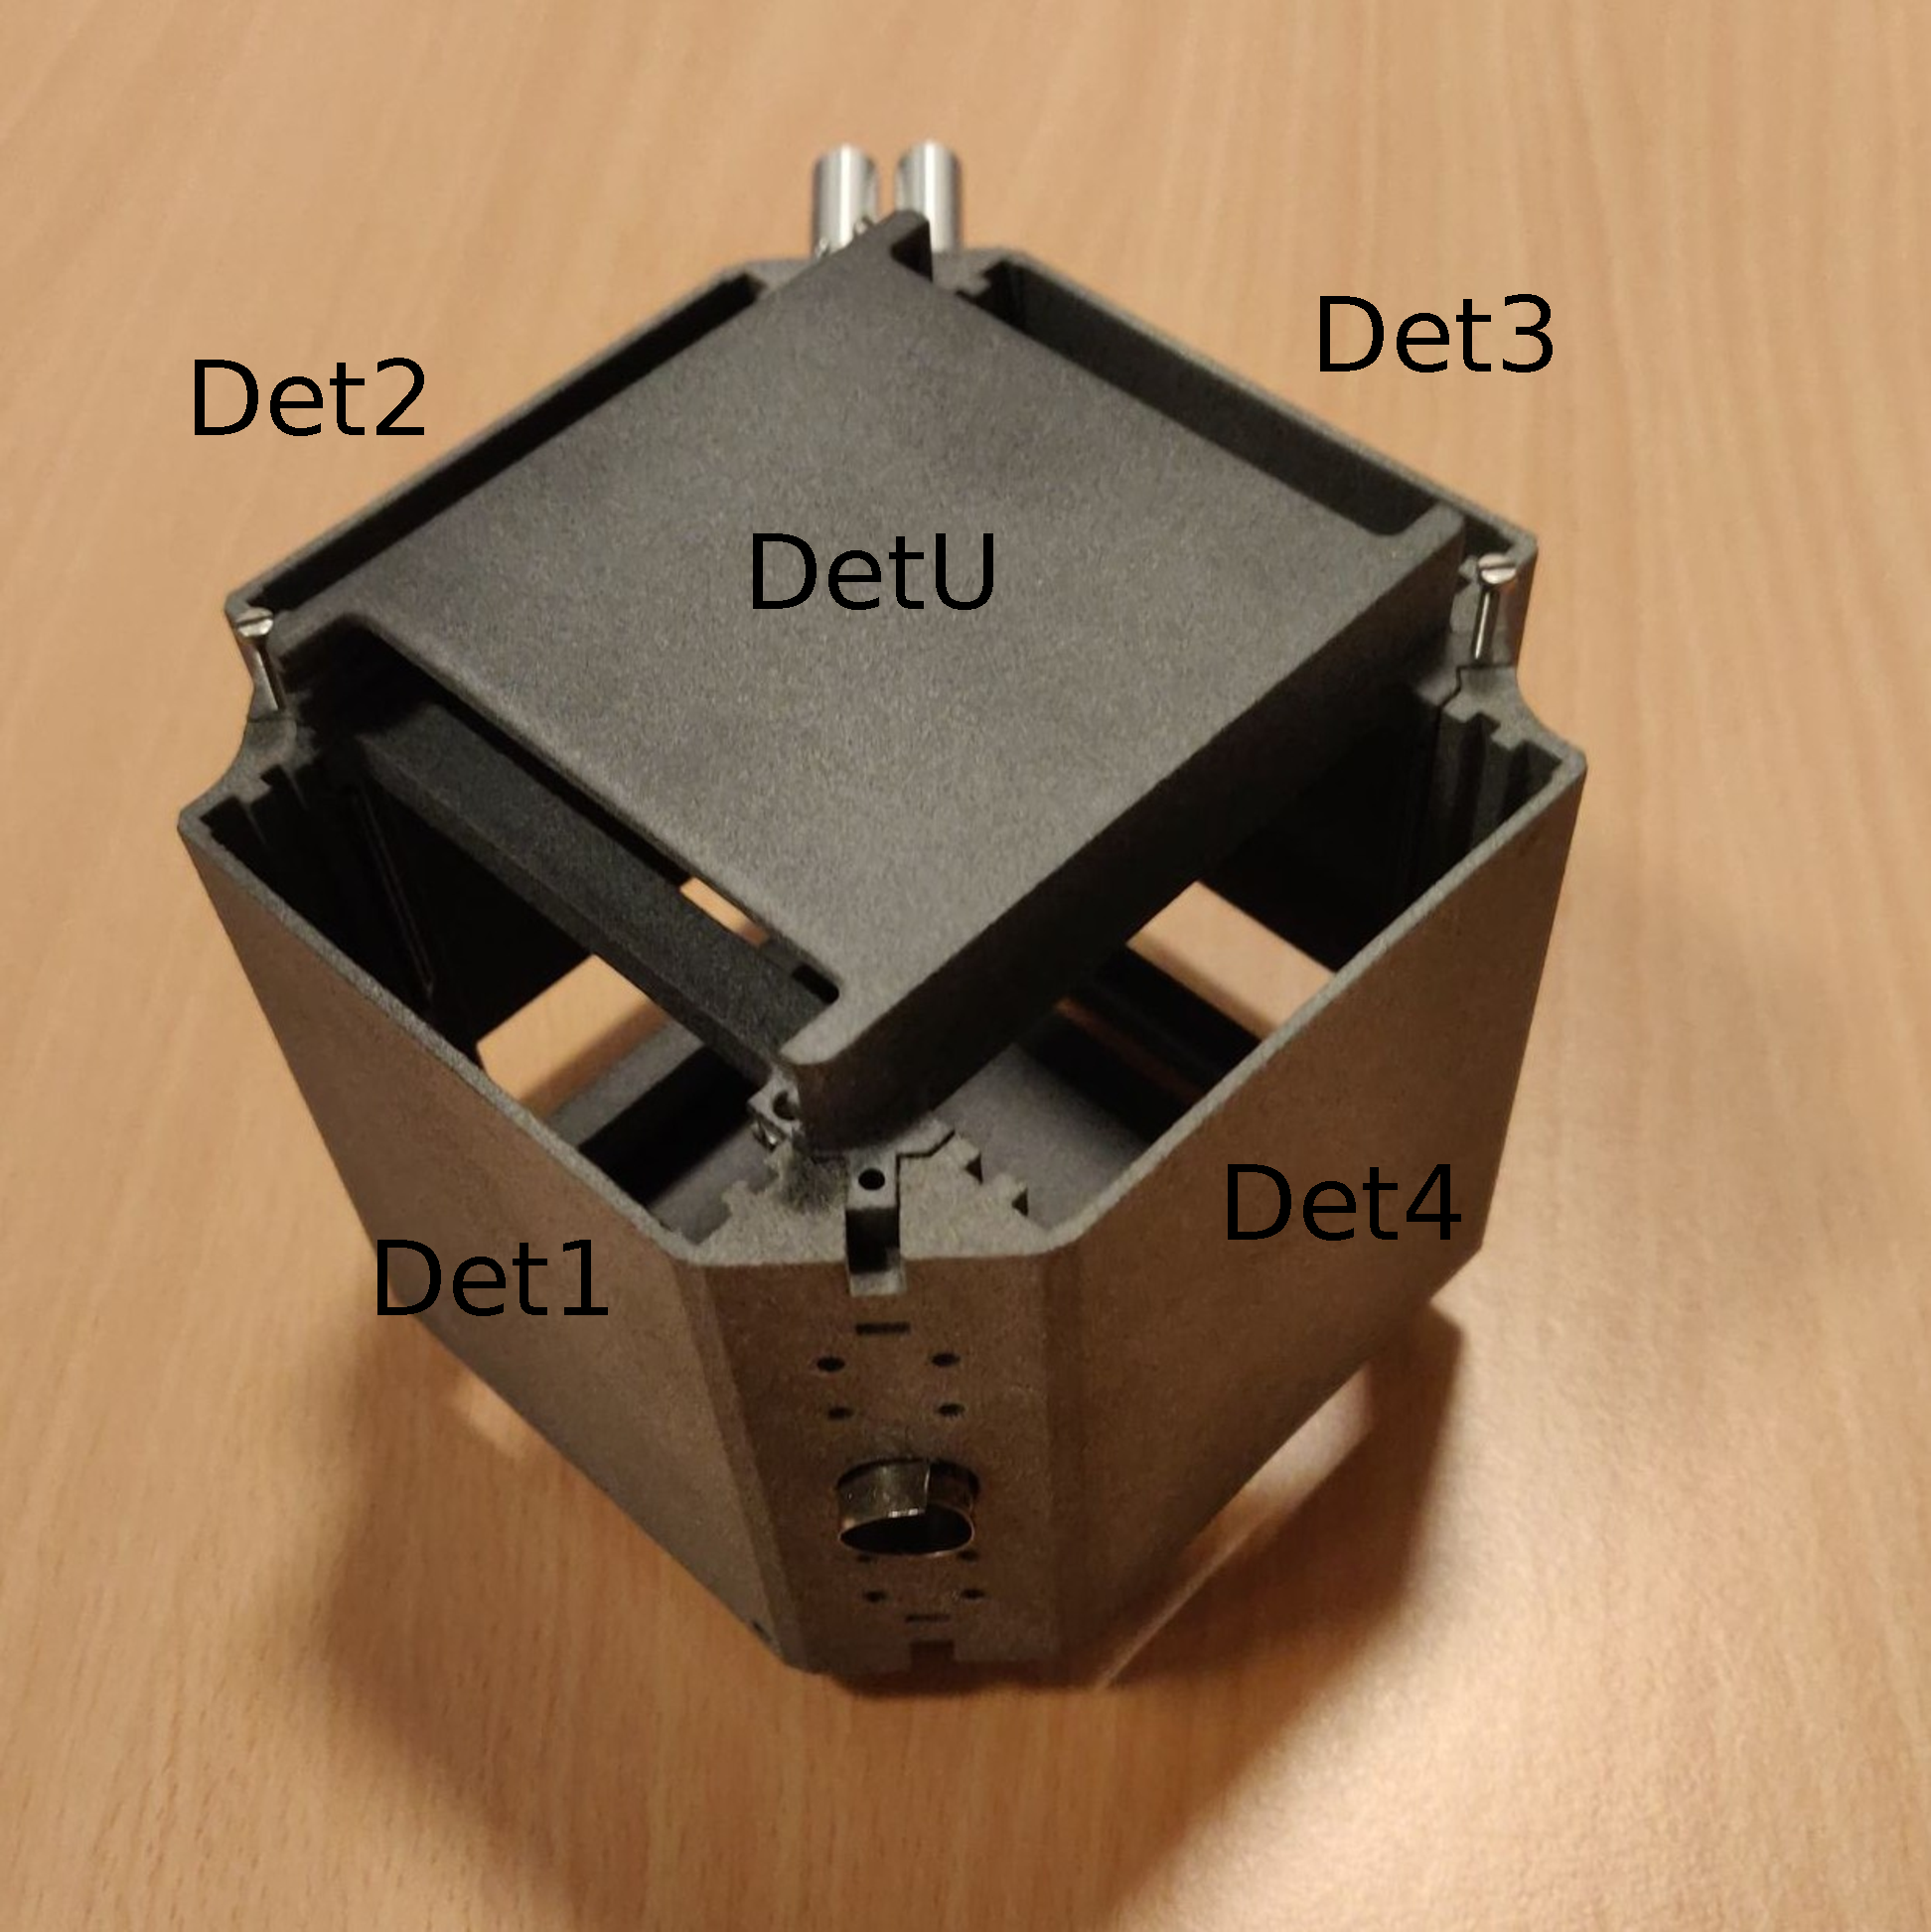
\includegraphics[width=\columnwidth]{../figures/cubepic.pdf}
		\end{figure}
		\column{0.49\textwidth}
		\begin{figure}
			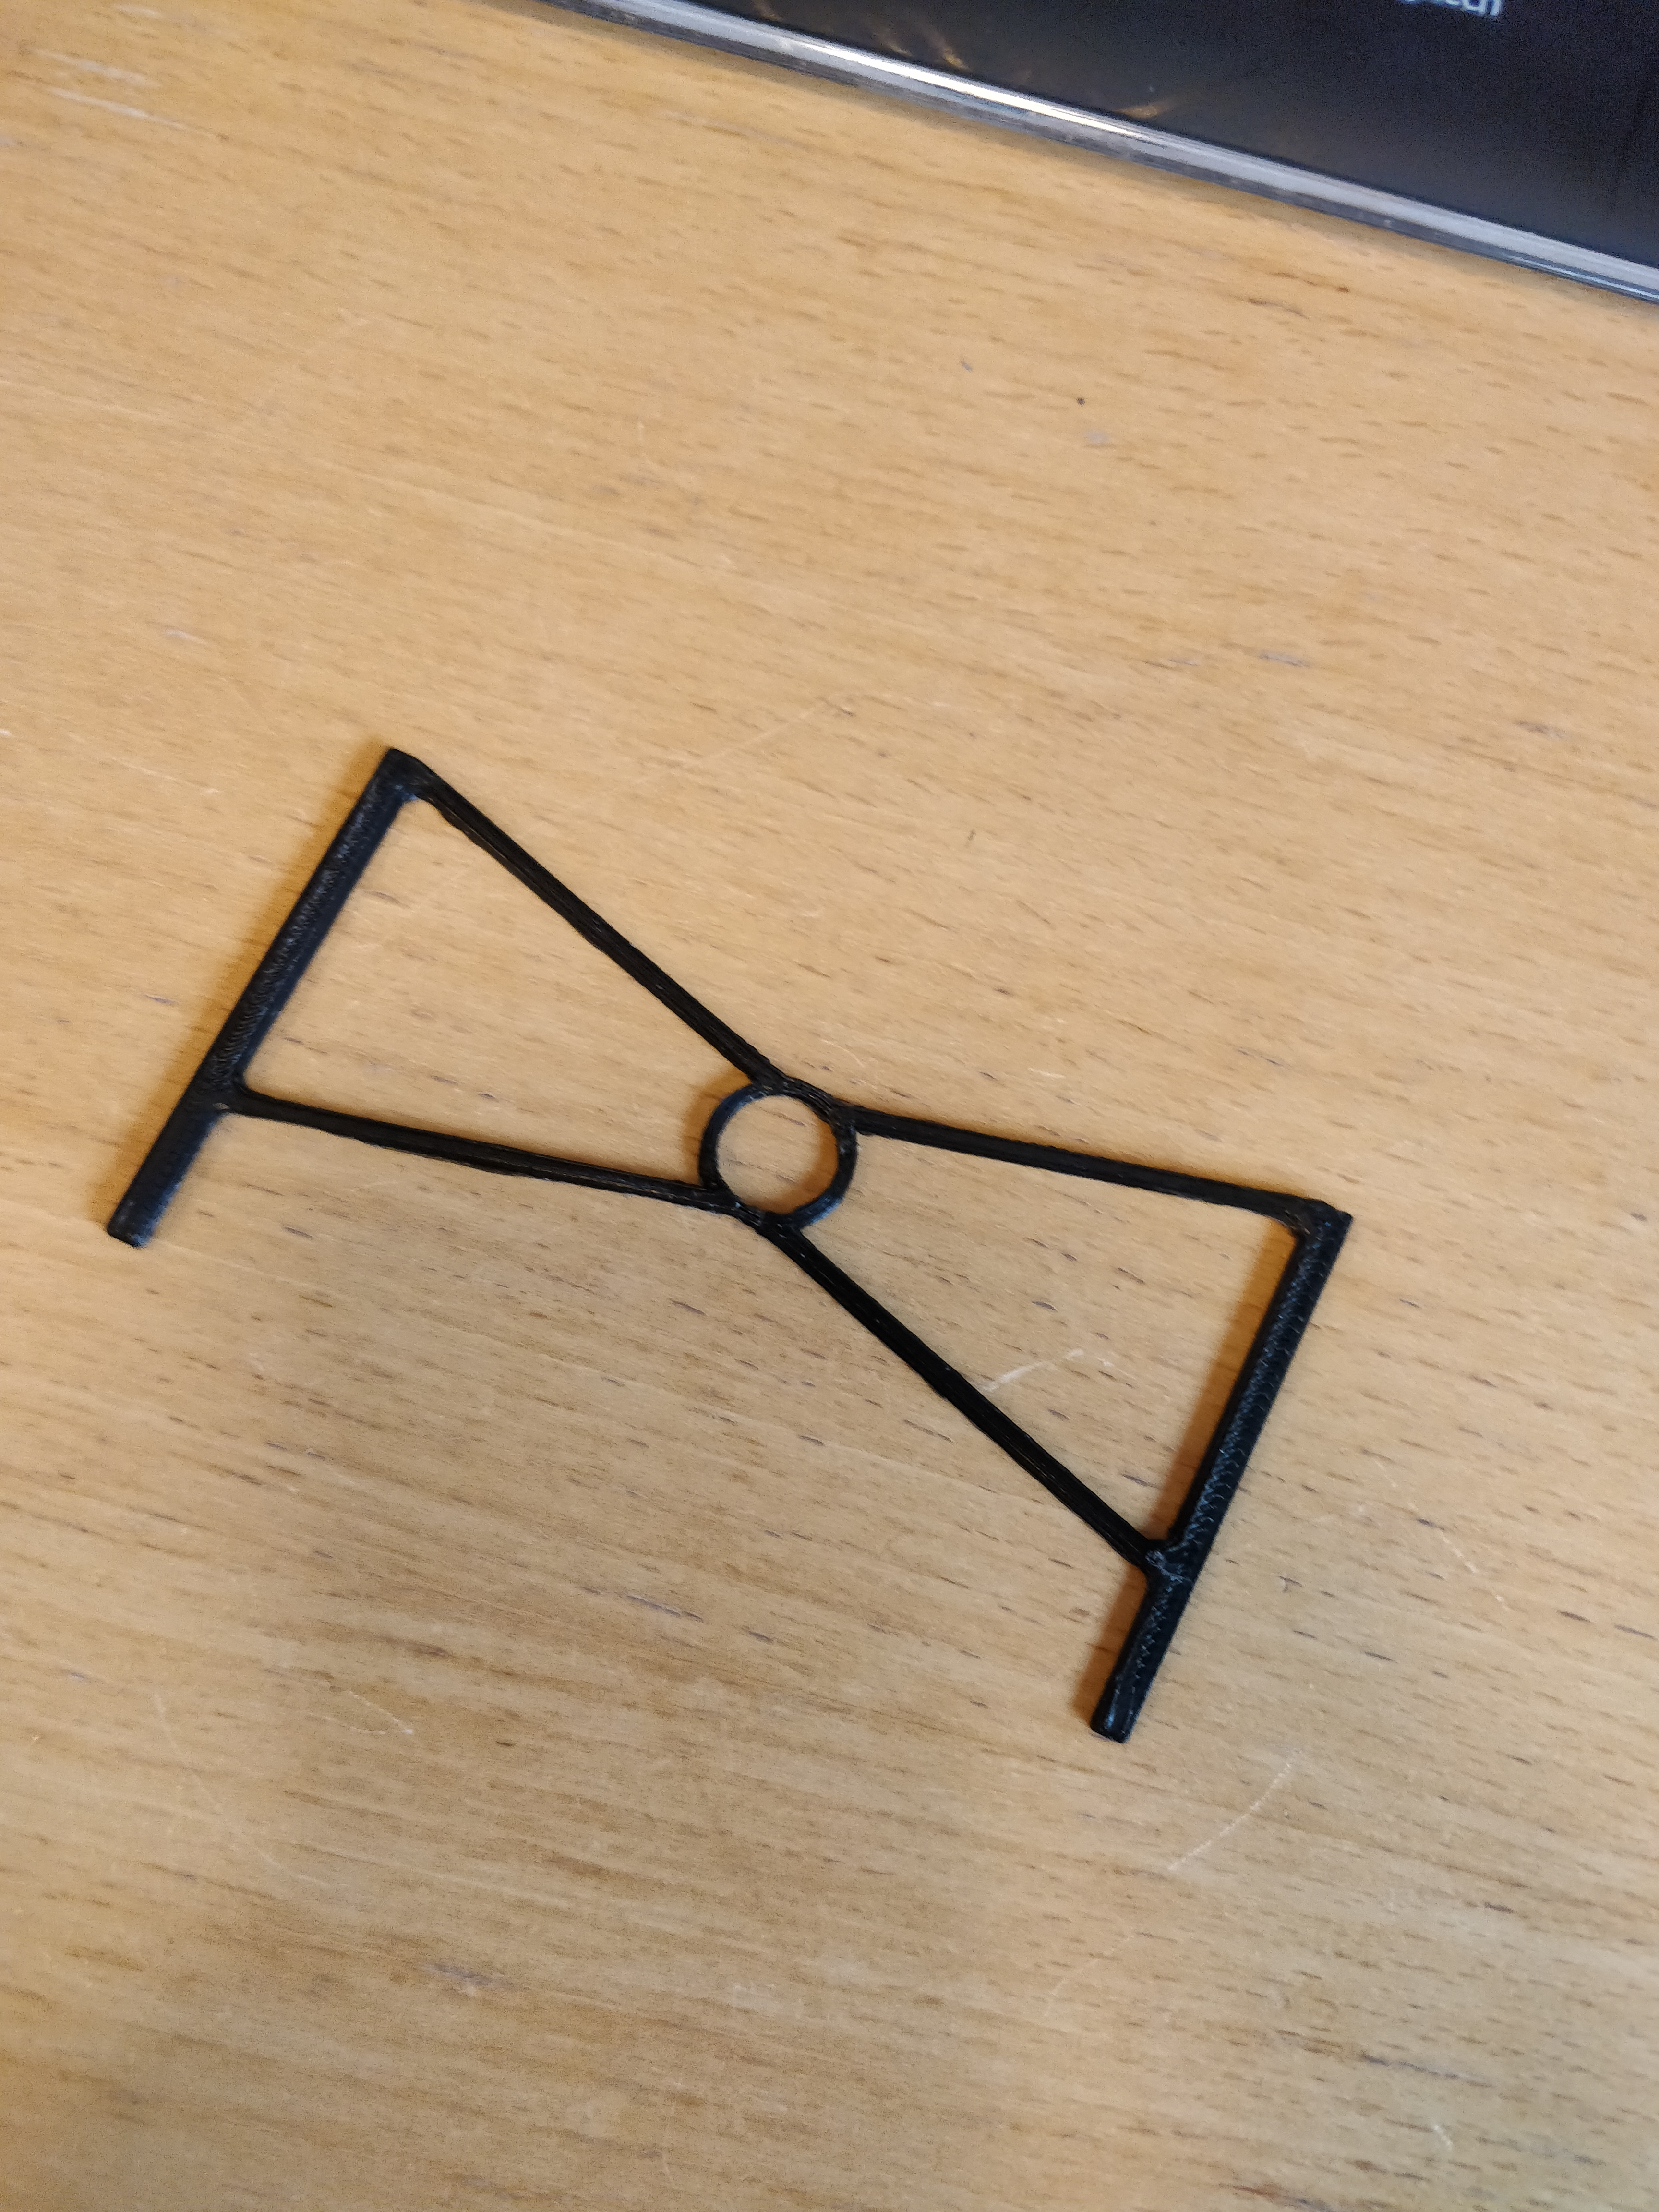
\includegraphics[width=.9\columnwidth]{../figures/targetHolder.jpg}
		\end{figure}
	\end{columns}
\end{frame}

\begin{frame}{Eksperimentel opsætning}
	\begin{columns}
		\column{0.4\textwidth}
		\begin{figure}
			\centering
			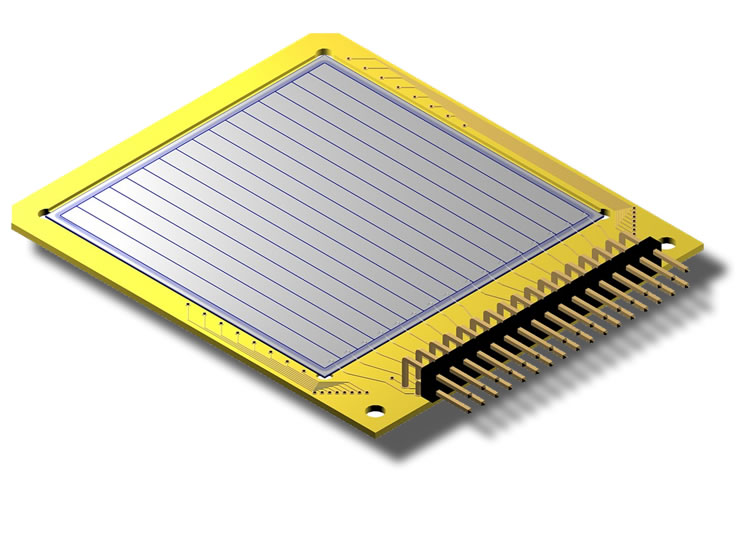
\includegraphics[width=\columnwidth]{../figures/W1.jpg}
		\end{figure}
		$16\times16$ strips\\
		256 pixels 
		\column{0.6\textwidth}
		\begin{figure}
			\centering
			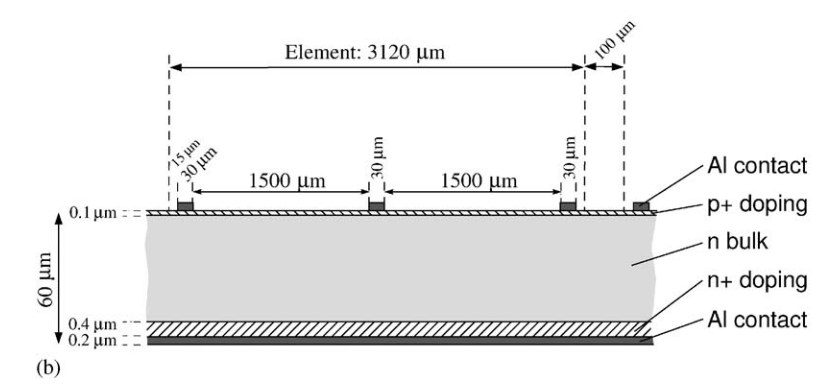
\includegraphics[width=\columnwidth]{../figures/dope.png}
		\end{figure}
	\end{columns}
\end{frame}

\begin{frame}{Software}
	\begin{columns}
		\column[]{0.6\textwidth}
	\begin{itemize}
		\onslide<2->{\item ROOT}
		\begin{itemize}
			\onslide<3->{\item C++ framework}
		\end{itemize}
		\onslide<4->{\item AUSA}
		\begin{itemize}
			\onslide<5->{\item Unpacker: Rå data til ROOT \texttt{Tree}}
			\onslide<6->{\item Calibrator: Detektor kalibrering}
			\onslide<7->{\item Sorter: Konvertere strip signaler til pixel hit}
		\end{itemize}
	\end{itemize}
	\column[]{0.4\textwidth}
	\onslide<7->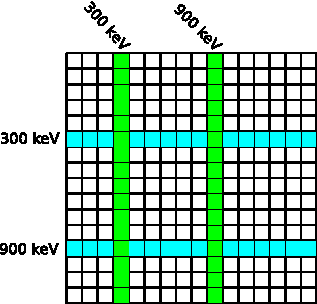
\includegraphics[width=\columnwidth]{../figures/sorter.pdf}
\end{columns}
\end{frame}

\begin{frame}{Kalibrering}
	\begin{columns}
		\column{0.5\textwidth}
		Kendte kilder:\\
		\begin{table}[H]
			\centering
			\begin{tabular}{ll}
				Isotope & $E_\alpha \ [keV]$  \\ \hline
				\isotope[148][]{Gd}		& 3182.690         \\
				\isotope[239][]{Pu}		& 5105.5           \\
				& 5144.3           \\
				& 5156.59          \\
				\isotope[244][]{Cm}		& 5762.64          \\
				& 5804.96          \\ 
			\end{tabular}
		\end{table}
	
		\column{0.5\textwidth}
		\begin{figure}
			\centering
			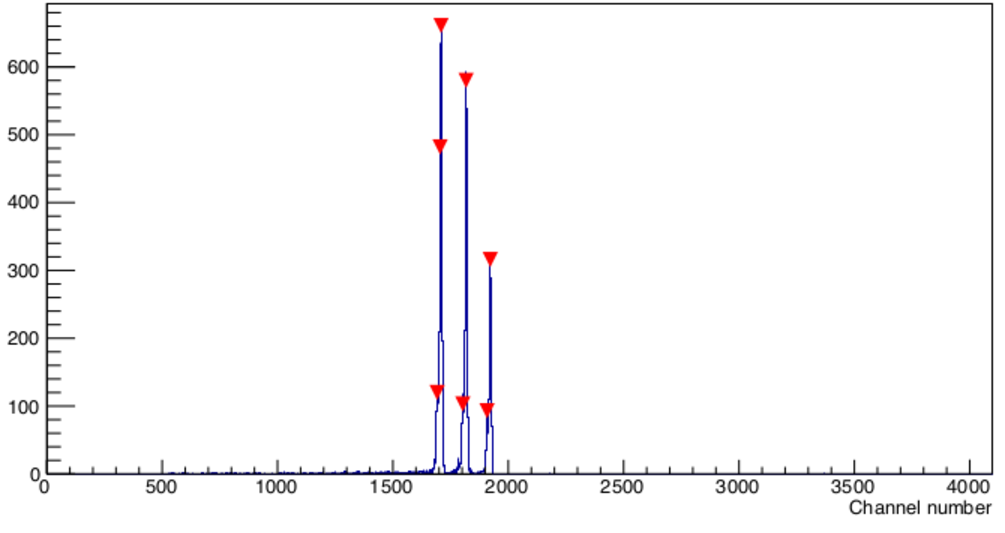
\includegraphics[width=\columnwidth]{../figures/cali/det1f1-cropped-Mia.pdf}
		\end{figure}
		\begin{figure}
			\centering
			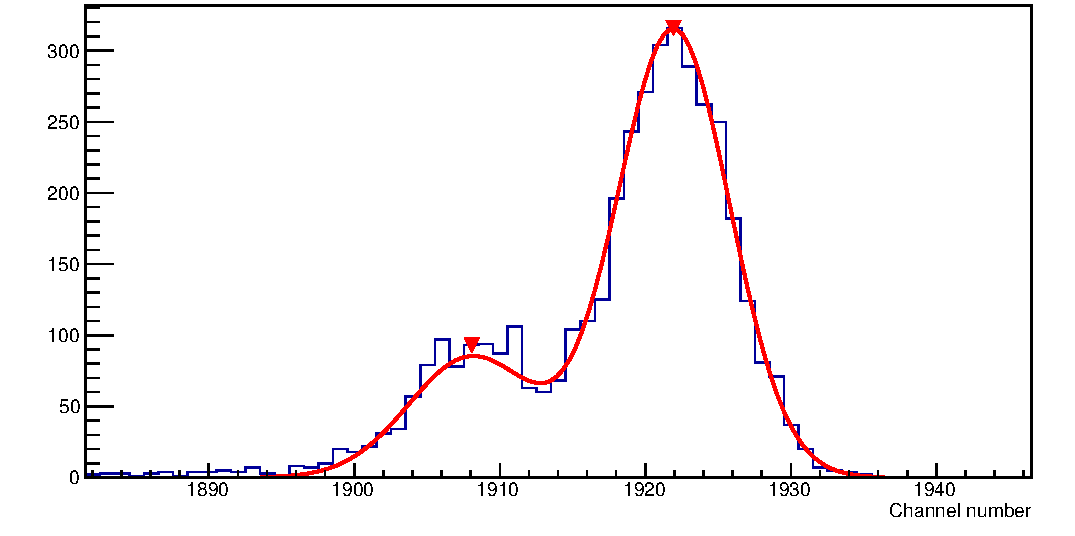
\includegraphics[width=\columnwidth]{../figures/cali/det1f1PeakMostLeft-cropped.pdf}
		\end{figure}
	\end{columns}
\end{frame}


\section{Data reduktion}

\begin{frame}{Identificer partikler}
	Forskellige energi afsætning\\
	\al-partikler bliver stoppet af \SI{60}{\mu m}\\
	\be-partikler afsætter \SI{300}{keV} - \SI{500}{keV} pr. mm silicium\\
	Overlappende energi\\
	\be-partikler bliver opfanget af PAD
\end{frame}

\begin{frame}{Identificer partikler}
	
\end{frame}

\end{document}